% =====================================================================
% WitnessRAG: método e desenho experimental (versão didática em português)
% Compilar: latexmk -pdf witnessrag-metodo-pt.tex
% Mesmo conteúdo e mesmas equações de witnessrag-method.tex, com intuição,
% leitura das fórmulas e exemplos em cada seção.
% =====================================================================
\documentclass[11pt]{article}
\usepackage[margin=2.3cm]{geometry}
\usepackage[T1]{fontenc}
\usepackage[utf8]{inputenc}
\usepackage[brazilian, provide=*]{babel}
\usepackage{amsmath,amssymb,amsthm}
\usepackage{booktabs,tabularx,array}
\usepackage{enumitem}

\usepackage{xcolor}
\usepackage[most]{tcolorbox}
\usepackage{tikz}
\usetikzlibrary{arrows.meta,positioning,fit,backgrounds,shapes.geometric,calc}
\usepackage{algorithm}
\usepackage{algpseudocode}
\usepackage[hidelinks]{hyperref}

\newtheorem{proposicao}{Proposição}
\newtheorem{definicao}{Definição}
\newtheorem{corolario}{Corolário}
\renewcommand{\proofname}{Demonstração}
\floatname{algorithm}{Algoritmo}
\renewcommand{\algorithmicrequire}{\textbf{Entrada:}}
\algrenewcommand\algorithmicif{\textbf{se}}
\algrenewcommand\algorithmicthen{\textbf{então}}
\algrenewcommand\algorithmicelse{\textbf{senão}}
\algrenewcommand\algorithmicend{\textbf{fim}}
\algrenewcommand\algorithmicreturn{\textbf{devolva}}

\newtcolorbox{intuicao}{enhanced, breakable, colback=blue!3, colframe=blue!45!black,
  title=Intuição, fonttitle=\bfseries\sffamily, boxrule=0.5pt, arc=2pt}
\newtcolorbox{empalavras}{enhanced, breakable, colback=gray!4, colframe=gray!55,
  coltitle=black, title=Lendo a fórmula em palavras, fonttitle=\bfseries\sffamily,
  boxrule=0.4pt, arc=2pt}
\newtcolorbox{exemplo}[1][]{enhanced, breakable, colback=green!3, colframe=green!40!black,
  title={Exemplo#1}, fonttitle=\bfseries\sffamily, boxrule=0.5pt, arc=2pt}
\newtcolorbox{nocodigo}{enhanced, breakable, colback=orange!3, colframe=orange!60!black,
  title=No código, fonttitle=\bfseries\sffamily, boxrule=0.4pt, arc=2pt}

\newcommand{\Compose}{\textsc{Compor}}
\newcommand{\Direct}{\textsc{Direta}}

\title{\textbf{WitnessRAG}\\[2pt]
\large Composição de testemunhas sob demanda para a memória de longo prazo de agentes\\[2pt]
\normalsize Método e desenho experimental: versão didática em português}
\author{}
\date{Versão de 23 de setembro de 2026}

\begin{document}
\maketitle

\begin{abstract}
Este texto é a versão em português da seção de método do artigo
(\texttt{witnessrag-method.tex}), reescrita para ser lida com calma. As
equações são as mesmas; cada seção traz primeiro a \emph{intuição}, depois a
definição formal, uma leitura da fórmula em palavras e um exemplo. A Seção~2
é uma visão geral detalhada, que acompanha perguntas reais do LoCoMo do
início ao fim. Onde um exemplo é ilustrativo (e não uma saída medida do
sistema), isso está dito explicitamente.
\end{abstract}

\tableofcontents
\newpage

% =====================================================================
\section*{Notação}
\addcontentsline{toc}{section}{Notação}

\begin{center}
\small
\begin{tabularx}{\textwidth}{@{}lX@{}}
\toprule
Símbolo & Significado \\
\midrule
$H=(s_1,\dots,s_T)$ & histórico: sequência de sessões de conversa \\
$u$ & uma fala (turno): locutor, texto e data \\
$\tau(u)$ & relógio de referência da fala: a data da sessão em que foi dita \\
$\mathcal{N}(u)$ & normalização de expressões relativas da fala (``ontem'' $\mapsto$ data) \\
$\mathcal{P}$ & conjunto de páginas (trechos de até 2.048 tokens) \\
$F$ & base de fatos extraídos; cada fato $f=(s,r,o,p,t,c)$ \\
$\Sigma$ & sinais de memória (relógio, ensaio, corroboração, excitação) \\
$\mathcal{M}=\langle\mathcal{P},F,\tau,\Sigma\rangle$ & a memória construída offline \\
$q$ & a pergunta \\
$k$ & orçamento de contexto: número de páginas entregues ao leitor ($k=5$) \\
$\mathcal{C}(q)$, $B_k(q)$ & pool híbrido de 20 candidatas e o seu top-$k$ \\
$C(q)$ & contexto final entregue ao leitor \\
$\pi(q)$ & contrato de evidência escrito pelo planejador \\
$\rho(\pi)$ & rota: \Direct{} ou \Compose{} \\
$Q(x)$ & consulta conjuntiva com variável de resposta $x$ \\
$\mathcal{W}_{Q,a}$ & testemunhas da resposta $a$ para a consulta $Q$ \\
$g(a,f)$ & escore de aterramento do átomo $a$ no fato $f$ \\
$y(q)$ & reflexão simbólica: $1$ se a junção produziu uma testemunha seletiva \\
$\Lambda$ & lentes de memória ligadas pelo contrato \\
$\Phi_T,\Phi_A,\Phi_C$ & lentes temporal, de saliência e de confiança \\
$\Gamma$ & métrica da tarefa (por exemplo, F1) com valores em $[0,1]$ \\
\bottomrule
\end{tabularx}
\end{center}

% =====================================================================
\section{Motivação e princípios}\label{sec:motivacao}

\begin{intuicao}
Imagine que um agente conversou com uma pessoa durante meses. Mais tarde,
alguém pergunta ``onde a Melanie já acampou?''. A resposta está espalhada em
três conversas diferentes. Guardar só um resumo das conversas perderia esses
detalhes; entregar tudo ao modelo de linguagem é caro e o confunde. O que se
quer é entregar ao leitor \emph{exatamente os trechos que demonstram a
resposta}, e só eles, dentro de um orçamento pequeno.
\end{intuicao}

\paragraph{Memória montada com antecedência versus sob demanda.}
Muitos sistemas de memória para agentes trabalham \emph{com antecedência}:
comprimem o histórico em resumos ou grafos e respondem a partir dessa versão
comprimida. Toda compressão perde informação, e o que se perdeu pode ser
justamente o que uma pergunta futura vai pedir. O General Agentic Memory
(GAM, Yan et al., 2025) propõe o princípio oposto, \emph{sob demanda}
(\emph{just-in-time}): um \textbf{memorizador} offline guarda o histórico
inteiro num repositório de páginas, e um \textbf{pesquisador} online, na hora
da pergunta, planeja, busca, integra e reflete até julgar que a informação
reunida basta.

\paragraph{O que o WitnessRAG muda.}
O WitnessRAG mantém essa divisão de trabalho, mas troca \emph{o que} o
pesquisador produz e \emph{como} ele decide que terminou. Em vez de um resumo
escrito por um modelo de linguagem e julgado suficiente por outro modelo, o
pesquisador tenta montar uma \textbf{testemunha}: um conjunto mínimo de fatos
armazenados que, juntos, implicam a resposta. Se essa testemunha existe ou
não é decidido por uma \emph{junção simbólica} sobre a memória de fatos, e
não por mais uma chamada ao modelo.

\paragraph{Três princípios.}
\begin{description}[leftmargin=1.2em, style=nextline]
\item[(P1) Planejar antes de buscar.] Uma única chamada de planejamento
descreve a necessidade de informação num vocabulário fechado e independente
de tarefa. Nenhum rótulo de benchmark é consultado. \emph{Por quê:} em
produção não existe rótulo ``esta pergunta é multi-hop''; o sistema precisa
entender sozinho o que está sendo pedido.
\item[(P2) Certificar o que pode ser certificado.] Perguntas cuja resposta é
uma conjunção de fatos armazenados são compostas e conferidas contra a
memória. Perguntas fora desse fragmento (cálculo de tempo, inferência
hipotética, sim/não) são servidas por recuperação e por sinais
especializados. \emph{Por quê:} não adianta pagar por uma prova quando a
pergunta não admite prova.
\item[(P3) Intervir com limites.] Toda intervenção edita um número fixo de
posições de um contexto híbrido forte. \emph{Por quê:} assim um erro do
planejador ou do executor tem custo limitado; no pior caso, perdem-se duas
das cinco páginas, e as três primeiras do híbrido estão sempre lá.
\end{description}

% =====================================================================
\section{Visão geral detalhada do processo}\label{sec:visao}

\begin{figure}[t]
\centering
\resizebox{\textwidth}{!}{%
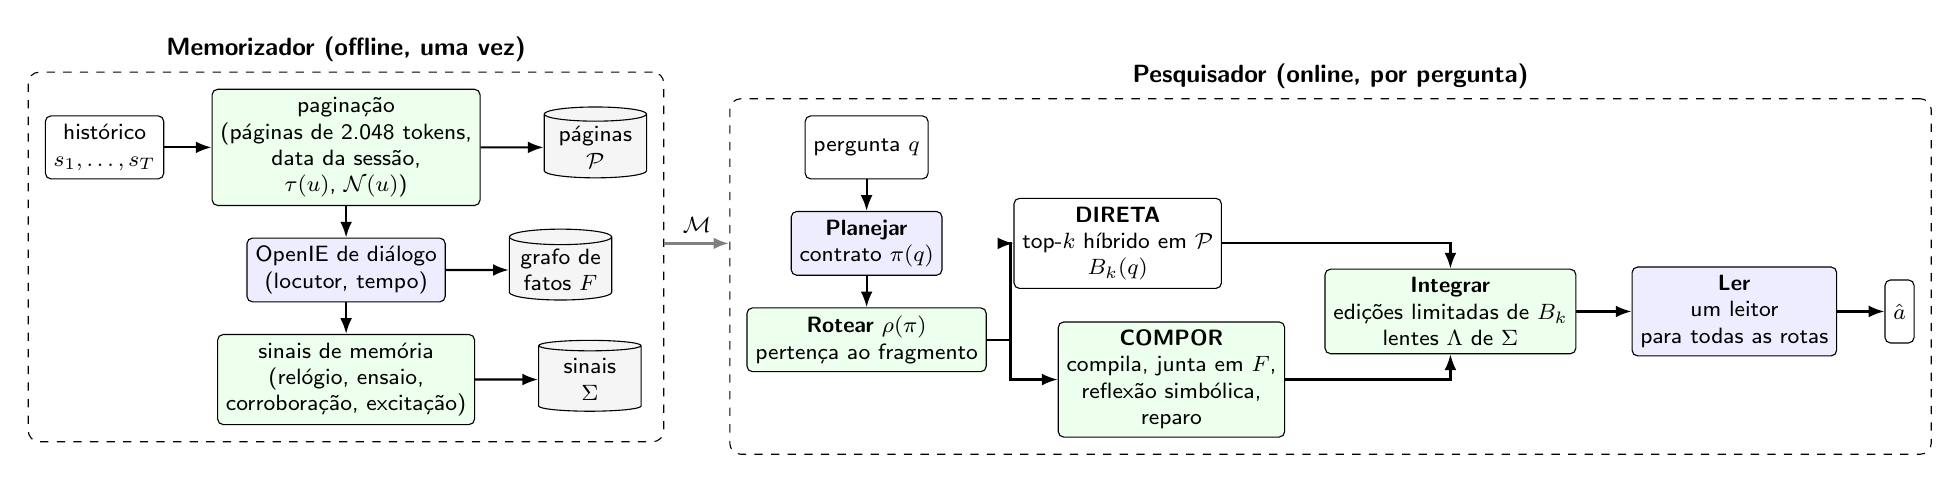
\begin{tikzpicture}[
  font=\sffamily\footnotesize, node distance=4mm and 6mm,
  box/.style={draw, rounded corners=2pt, align=center, minimum height=8mm,
              inner sep=3pt, fill=white},
  store/.style={draw, cylinder, shape border rotate=90, aspect=0.18,
                minimum height=9mm, minimum width=13mm, align=center,
                inner sep=1pt, fill=gray!8},
  llm/.style={box, fill=blue!7},
  sym/.style={box, fill=green!7},
  arr/.style={-{Latex[length=2mm]}, thick},
  grp/.style={draw, dashed, rounded corners=4pt, inner sep=6pt},
]
\node[box] (hist) {histórico\\$s_1,\dots,s_T$};
\node[sym, right=of hist] (page) {paginação\\(páginas de 2.048 tokens,\\data da sessão,\\$\tau(u)$, $\mathcal{N}(u)$)};
\node[llm, below=of page] (ie) {OpenIE de diálogo\\(locutor, tempo)};
\node[sym, below=of ie] (sig) {sinais de memória\\(relógio, ensaio,\\corroboração, excitação)};
\node[store, right=8mm of page] (P) {páginas\\$\mathcal{P}$};
\node[store, right=8mm of ie] (F) {grafo de\\fatos $F$};
\node[store, right=8mm of sig] (S) {sinais\\$\Sigma$};
\draw[arr] (hist) -- (page);
\draw[arr] (page) -- (P);
\draw[arr] (page) -- (ie);
\draw[arr] (ie) -- (F);
\draw[arr] (ie) -- (sig);
\draw[arr] (sig) -- (S);
\begin{scope}[on background layer]
  \node[grp, fit=(hist)(page)(ie)(sig)(P)(F)(S), label={[font=\sffamily\small\bfseries]above:Memorizador (offline, uma vez)}] (mem) {};
\end{scope}
\node[box, right=20mm of P] (q) {pergunta $q$};
\node[llm, below=of q] (plan) {\textbf{Planejar}\\contrato $\pi(q)$};
\node[sym, below=of plan] (route) {\textbf{Rotear} $\rho(\pi)$\\pertença ao fragmento};
\node[box, right=9mm of plan] (direct) {\textbf{DIRETA}\\top-$k$ híbrido em $\mathcal{P}$\\$B_k(q)$};
\node[sym, right=9mm of sig -| route.east, anchor=west] (compose) {\textbf{COMPOR}\\compila, junta em $F$,\\reflexão simbólica,\\reparo};
\coordinate (mid) at ($(direct.east)!0.5!(compose.east)$);
\node[sym, anchor=west] (integ) at ($(mid)+(9mm,0)$) {\textbf{Integrar}\\edições limitadas de $B_k$\\lentes $\Lambda$ de $\Sigma$};
\node[llm, right=7mm of integ] (read) {\textbf{Ler}\\um leitor\\para todas as rotas};
\node[box, right=6mm of read] (ans) {$\hat a$};
\draw[arr] (q) -- (plan);
\draw[arr] (plan) -- (route);
\draw[arr] (route.east) -- ++(3mm,0) |- (direct.west);
\draw[arr] (route.east) -- ++(3mm,0) |- (compose.west);
\draw[arr] (direct.east) -| (integ.north);
\draw[arr] (compose.east) -| (integ.south);
\draw[arr] (integ) -- (read);
\draw[arr] (read) -- (ans);
\begin{scope}[on background layer]
  \node[grp, fit=(q)(plan)(route)(direct)(compose)(integ)(read)(ans), label={[font=\sffamily\small\bfseries]above:Pesquisador (online, por pergunta)}] (res) {};
\end{scope}
\draw[arr, very thick, gray] (mem.east |- plan) -- node[above, black] {$\mathcal{M}$} (res.west |- plan);
\end{tikzpicture}}
\caption{Visão geral. O memorizador guarda todas as falas em páginas e deriva
um grafo de fatos e sinais de memória. Para cada pergunta, o pesquisador
escreve um contrato de evidência, escolhe a rota pela pertença ao fragmento,
compõe testemunhas quando a necessidade é conjuntiva, edita poucas posições do
contexto híbrido e chama um único leitor. Azul: chamadas ao modelo de
linguagem; verde: passos simbólicos, sem modelo.}
\label{fig:visao}
\end{figure}

\subsection{As duas fases}

O sistema tem duas fases (Figura~\ref{fig:visao}). A \textbf{fase offline}
acontece uma vez por memória: o memorizador transforma o histórico em
$\mathcal{M}=\langle\mathcal{P},F,\tau,\Sigma\rangle$. A \textbf{fase online}
acontece a cada pergunta: o pesquisador percorre a memória e entrega um
contexto de $k=5$ páginas ao leitor. A Tabela~\ref{tab:etapas} resume cada
etapa com a sua entrada, a sua saída e o seu custo.

\begin{table}[h]
\centering
\small
\caption{Etapas do WitnessRAG. ``LLM'' indica chamada ao modelo de linguagem.}
\label{tab:etapas}
\begin{tabularx}{\textwidth}{@{}l>{\raggedright}X>{\raggedright}Xl@{}}
\toprule
Etapa & Entrada & Saída & LLM? \\
\midrule
\multicolumn{4}{@{}l}{\emph{Offline (uma vez por memória)}}\\
Paginação & histórico $H$ & páginas $\mathcal{P}$ com $\tau(u)$ e $\mathcal{N}(u)$ & não \\
Extração & janelas de 512 tokens & fatos $F$ com locutor e tempo & 2 por janela \\
Canonização & fatos & clusters de identidade, famílias de relação & não \\
Sinais & $\mathcal{P}$, $F$ & relógio, ensaio, corroboração & não \\
\midrule
\multicolumn{4}{@{}l}{\emph{Online (por pergunta)}}\\
Recuperação base & $q$ & pool $\mathcal{C}(q)$ (20) e $B_k(q)$ (5) & não \\
Planejar & texto de $q$ & contrato $\pi(q)$ & 1 \\
Rotear & $\pi(q)$ & \Direct{} ou \Compose{} & não \\
Compilar & $q$, vocabulário do grafo & consulta conjuntiva $Q$ & 1, só em \Compose{} \\
Aterrar e juntar & $Q$, $F$ & testemunhas, respostas, lacuna & não \\
Refletir & resultado da junção & $y(q)\in\{0,1\}$ & não \\
Reparar & $Q$ ou a lacuna & no máximo 1 página nova & não \\
Lentes & $\pi$, $\Sigma$, pool & no máximo $L$ trocas & não \\
Ler & $q$, $C(q)$ & resposta curta $\hat a$ & 1 \\
\bottomrule
\end{tabularx}
\end{table}

\subsection{O percurso de uma pergunta, passo a passo}\label{sec:passos}

\begin{enumerate}[label=\textbf{Passo \arabic*.}, leftmargin=*, align=left]
\setcounter{enumi}{-1}
\item \textbf{Recuperação base.} A pergunta é buscada por similaridade densa
(BGE-M3) e por palavras-chave (BM25). As duas listas são fundidas por
\emph{reciprocal rank fusion} num pool $\mathcal{C}(q)$ de 20 páginas; as 5
primeiras formam $B_k(q)$. \emph{Se tudo o mais falhar, é isto que o leitor
vê.} Todo o resto do método é uma edição de poucas posições do fim de $B_k$.

\item \textbf{Planejar.} Uma chamada ao modelo lê \emph{somente o texto da
pergunta} e escreve o contrato $\pi(q)$: que forma tem a resposta, que
raciocínio vem depois da busca, se a evidência está num lugar ou em vários, se
há foco temporal, quem são as entidades, o que procurar e quais sinais de
memória usar. \emph{Se o contrato vier inválido ou for bloqueado pelo filtro
de conteúdo}, ele vale $\bot$ e a pergunta segue pela rota \Direct{}.

\item \textbf{Rotear.} Uma regra fixa lê o contrato e decide: \Compose{} se a
necessidade cabe no fragmento que o executor sabe provar e envolve vários
fatos; \Direct{} caso contrário. Não há chamada ao modelo aqui.

\item \textbf{Rota \Direct{}.} O contexto é $B_k(q)$. Nada mais acontece antes
das lentes.

\item \textbf{Rota \Compose{}.} (a) Uma segunda chamada compila a pergunta
numa consulta conjuntiva $Q$. (b) Cada átomo de $Q$ recebe fatos candidatos
(aterramento). (c) Uma busca em feixe monta atribuições consistentes das
variáveis e extrai testemunhas mínimas (junção). (d) A \emph{reflexão
simbólica} $y(q)$ verifica se a junção é seletiva o bastante. (e) Se $y(q)=1$,
as páginas das testemunhas entram nas duas últimas posições. Se $y(q)=0$, há
no máximo um reparo: uma página recuperada por pelo menos duas sondas
diferentes, ou a página que fecha a lacuna da junção, entra na última
posição. Se nada disso acontece, o contexto continua $B_k(q)$.

\item \textbf{Lentes (opcional).} Se o contrato ligou lentes (temporal,
saliência, confiança), elas podem trocar até $L$ páginas não protegidas da
cauda por outras do pool. Páginas colocadas pela rota \Compose{} são
protegidas.

\item \textbf{Integrar.} O resultado é $C(q)$, que difere de $B_k(q)$ em no
máximo $\max(2,L)$ posições.

\item \textbf{Ler.} Um único leitor, igual para todas as rotas e todos os
métodos comparados, lê $q$ e $C(q)$ numa visão temporal (cada fala com a sua
data e a normalização de ``ontem'', ``semana passada'') e devolve uma
resposta curta.
\end{enumerate}

\subsection{Três perguntas reais acompanhadas do início ao fim}\label{sec:exemplos}

Os textos das falas e as respostas abaixo são do LoCoMo (conversa
\texttt{conv-26}). Os contratos e as consultas mostrados são
\textbf{ilustrativos}: indicam o que o mecanismo faz com essas entradas, não
saídas medidas do modelo.

\begin{exemplo}[ 1: uma pergunta de tempo (rota \Direct{})]
\textbf{Pergunta:} ``When did Caroline go to the LGBTQ support group?''
\textbf{Resposta de referência:} 7 May 2023.

\textbf{Memória.} A fala relevante está na primeira sessão:
\begin{quote}\small\ttfamily
Session date: 1:56 pm on 8 May, 2023\\
{[D1:3]} Caroline: I went to a LGBTQ support group yesterday and it was so powerful.\\
{[D1:3 temporal]} reference\_time=2023-05-08; "yesterday"=7 May 2023
\end{quote}
A terceira linha é a normalização $\mathcal{N}(u)$ calculada offline, sem
modelo: ``yesterday'' relativo a $\tau(u)=$ 8/5/2023 vira 7/5/2023.

\textbf{Planejar.} Contrato: forma \emph{time}, operador \emph{temporal},
escopo \emph{single}, foco temporal \emph{when}.
\textbf{Rotear.} O operador é temporal: fora do fragmento conjuntivo. Rota
\Direct{}.
\textbf{Ler.} O leitor recebe $B_k(q)$ na visão temporal e encontra a linha
normalizada. A resposta ``7 May 2023'' não exige calcular a data: ela já está
escrita na página. \emph{Custo: 2 chamadas.}
\end{exemplo}

\begin{exemplo}[ 2: uma pergunta de conjunto (rota \Compose{})]
\textbf{Pergunta:} ``Where has Melanie camped?''
\textbf{Resposta de referência:} beach, mountains, forest.

\textbf{Memória.} Os três itens estão em três sessões diferentes:
\begin{quote}\small
\texttt{[D4:6]} (27/6/2023) Melanie: ``\dots I just took my fam camping in the mountains last week\dots''\\
\texttt{[D6:16]} (6/7/2023) Melanie: ``\dots Here's a pic of my family camping at the beach\dots''\\
\texttt{[D8:32]} (15/7/2023) Melanie: ``\dots We even went on another camping trip in the forest.''
\end{quote}

\textbf{Planejar.} Contrato: forma \emph{set}, operador \emph{aggregate},
escopo \emph{multiple}.
\textbf{Rotear.} Agregação de vários fatos com resposta de entidades: rota
\Compose{}.
\textbf{Compilar.} $Q(x)=\mathrm{camp}(\text{Melanie},x)$, agregação
\emph{set}.
\textbf{Juntar.} Se o extrator produziu os fatos
$f_1=(\text{Melanie},\text{camp in},\text{mountains})$,
$f_2=(\text{Melanie},\text{camp at},\text{beach})$ e
$f_3=(\text{Melanie},\text{camp in},\text{forest})$, cada um é, sozinho, uma
testemunha de um membro: $\{f_1\}$ para \emph{mountains}, $\{f_2\}$ para
\emph{beach}, $\{f_3\}$ para \emph{forest}. O conjunto de respostas é
$A=\{\text{mountains},\text{beach},\text{forest}\}$, com $|A|=3$.
\textbf{Refletir.} $|A|\le3$ e há uma testemunha por resposta; se a busca não
foi truncada e o suporte da melhor resposta passa de $0{,}45$, as páginas
dessas testemunhas entram no contexto, até o limite de duas páginas.
\textbf{Ler.} O leitor lista todos os itens sustentados pelas páginas.

\textbf{Por que isto importa.} A métrica oficial do LoCoMo para esta categoria
dá a cada item de referência o melhor casamento entre os itens previstos. Uma
resposta com um só item fica limitada a cerca de $1/3$ de F1. Garantir que as
páginas de \emph{todos} os membros estejam no contexto é o que a composição
oferece a mais que a busca por similaridade.
\end{exemplo}

\begin{exemplo}[ 3: uma pergunta hipotética (rota \Direct{})]
\textbf{Pergunta:} ``Would Caroline pursue writing as a career option?''
\textbf{Resposta de referência:} ``Likely no; though she likes reading, she
wants to be a counselor''.

\textbf{Planejar.} Contrato: forma \emph{yes\_no}, operador \emph{abduce}.
\textbf{Rotear.} A resposta não é derivável de fatos armazenados (é uma
inferência provável), portanto não existe testemunha: rota \Direct{}.
\textbf{Ler.} O leitor combina o que as páginas dizem (Caroline quer ser
conselheira) com conhecimento comum e responde ``likely no''.
\end{exemplo}

% =====================================================================
\section{Formulação do problema}\label{sec:problema}

\begin{intuicao}
Temos um histórico longo e um orçamento pequeno: só $k=5$ páginas podem ir
para o leitor. O problema é escolher \emph{quais} cinco, pergunta a pergunta,
gastando poucas chamadas ao modelo. A formulação abaixo diz isso com
precisão e introduz o objeto central do método, a testemunha.
\end{intuicao}

\paragraph{Histórico, memória e contexto.}
Um histórico é uma sequência de sessões $H=(s_1,\dots,s_T)$. Cada fala $u$
tem um locutor, um texto e um relógio de referência $\tau(u)$, a data da sua
sessão. O memorizador transforma $H$ numa memória $\mathcal{M}$. Para uma
pergunta $q$, o pesquisador devolve um contexto $C(q)\subseteq\mathcal{P}$
com exatamente $k$ páginas, e um leitor produz a resposta
$\hat a=\mathrm{Read}(q,C(q))$. Como no GAM, o objetivo é o desempenho na
tarefa sob um orçamento fixo de contexto:
\begin{equation}
  C^\star(q)\in\arg\max_{C\subseteq\mathcal{P},\,|C|=k}
  \;\mathbb{E}\bigl[\Gamma(\mathrm{Read}(q,C))\bigr].
  \label{eq:objetivo}
\end{equation}
Além disso, limitamos o número de chamadas ao modelo por pergunta
(Seção~\ref{sec:custo}).

\begin{empalavras}
Entre todos os conjuntos de $k$ páginas possíveis, queremos o que faz o
leitor acertar mais, em média ($\mathbb{E}$ porque o leitor pode variar).
$\Gamma$ é a métrica (por exemplo F1). Não sabemos resolver isso exatamente:
seria preciso testar todos os subconjuntos. O WitnessRAG é uma estratégia para
aproximar $C^\star$ com uma estrutura lógica.
\end{empalavras}

\paragraph{Consultas conjuntivas.}
Uma consulta conjuntiva positiva com variável de resposta $x$ é
\begin{equation}
  Q(x)\;=\;\exists\,\bar y\;\bigwedge_{j=1}^{m} r_j(t_j, t'_j),
  \label{eq:cq}
\end{equation}
em que cada termo $t_j,t'_j$ é uma constante (um nome) ou uma variável.

\begin{empalavras}
``Existe um valor para as variáveis intermediárias $\bar y$ tal que todas as
$m$ relações valem ao mesmo tempo.'' Cada $r_j(t_j,t'_j)$ é um \emph{átomo}:
uma relação entre dois termos. O símbolo $\bigwedge$ é um ``e'' repetido.
\end{empalavras}

\begin{exemplo}[: três formas de consulta]
Fatos: $e_1$ Ana trabalha na Atlas; $e_2$ Atlas fica em Recife;
$e_3$ Ana pesquisa Óptica; $e_4$ Bruno trabalha na Atlas; $e_5$ Bruno
pesquisa Óptica.
\begin{itemize}[nosep]
\item Um átomo: $Q_1(x)=\mathrm{trabalhaEm}(\text{Ana},x)$. Resposta: Atlas.
\item Cadeia: $Q_2(x)=\exists y\;\mathrm{trabalhaEm}(\text{Ana},y)\wedge\mathrm{ficaEm}(y,x)$. Resposta: Recife.
\item Interseção: $Q_3(x)=\mathrm{trabalhaEm}(x,\text{Atlas})\wedge\mathrm{pesquisa}(x,\text{Óptica})$. Respostas: Ana e Bruno.
\end{itemize}
Em $Q_3$ a \emph{mesma} pessoa precisa satisfazer os dois átomos. Recuperar
``alguém da Atlas'' e ``outra pessoa que pesquisa Óptica'' não responde nada.
É isso que distingue uma junção de uma lista de trechos relevantes.
\end{exemplo}

\paragraph{Testemunhas.}
\begin{definicao}[Testemunha]
Dada uma base de fatos $F$, uma consulta $Q$ e uma resposta $a$, as
testemunhas de $a$ são os subconjuntos de $F$ mínimos por inclusão que
implicam $Q(a)$:
\begin{equation}
  \mathcal{W}_{Q,a}=\bigl\{\,W\subseteq F \;:\; W\models Q(a),\;
  \forall W'\subsetneq W,\;W'\not\models Q(a)\bigr\}.
  \label{eq:testemunha}
\end{equation}
\end{definicao}

\begin{empalavras}
$W\models Q(a)$ lê-se ``os fatos de $W$ bastam para demonstrar que $a$
responde $Q$''. A segunda condição diz que nenhum fato de $W$ sobra: tirando
qualquer um, a demonstração quebra. ``Mínimo por inclusão'' não quer dizer
``menor tamanho'': uma resposta pode ter várias testemunhas de tamanhos
diferentes.
\end{empalavras}

\begin{proposicao}[Testemunhas caracterizam respostas]\label{prop:caracterizacao}
Para qualquer memória retida $S\subseteq F$, finita, e consulta conjuntiva
positiva $Q$:
\[
a\in\mathrm{Ans}(Q,S)\iff \exists\,W\in\mathcal{W}_{Q,a}\ \text{com}\ W\subseteq S.
\]
\end{proposicao}
\begin{proof}
($\Leftarrow$) Se $W\subseteq S$ e $W\models Q(a)$, então $S\models Q(a)$,
porque a consulta é positiva (mais fatos não desfazem uma demonstração).
($\Rightarrow$) Se $a\in\mathrm{Ans}(Q,S)$, existe uma atribuição das
variáveis que torna cada átomo verdadeiro por algum fato de $S$; esses fatos
formam um conjunto finito que implica $Q(a)$. Retirando fatos redundantes um
a um, chega-se a um conjunto mínimo, que é uma testemunha contida em $S$.
\end{proof}

\paragraph{Consequências.}
(i) Preservar e recuperar respostas \emph{é o mesmo que} preservar e
recuperar testemunhas. (ii) Juntando todas as testemunhas de $a$, obtém-se o
seu \emph{polinômio de proveniência} (Green et al., 2007):
$a\Leftarrow\bigvee_{W\in\mathcal{W}_{Q,a}}\bigwedge_{f\in W}f$, um ``ou'' de
``e''s; cada testemunha é um monômio. (iii) Numa consulta de um átomo
($m=1$), a testemunha é um único fato, que mora numa única página; um bom
recuperador já encontra essa página. A composição importa quando $m\ge2$ ou
quando a resposta é o \emph{conjunto} de todos os $a$ com testemunha.

% =====================================================================
\section{Memorizador: uma memória pronta para testemunhas}\label{sec:memorizador}

\begin{intuicao}
Antes de qualquer pergunta, o memorizador organiza o histórico de três
formas complementares: o texto integral (para o leitor), fatos estruturados
(para a junção) e estatísticas simples (para as lentes). Nada nesta fase olha
para perguntas ou respostas.
\end{intuicao}

\paragraph{Paginação.}
O histórico é cortado em páginas de até 2.048 tokens, como no repositório de
páginas do GAM. Cada página começa com o cabeçalho da sessão, e cada fala
carrega o seu relógio $\tau(u)$. Um normalizador determinístico $\mathcal{N}$
converte expressões relativas em valores absolutos ancorados em $\tau(u)$:
``yesterday'' $\mapsto\tau(u)-1$ dia; ``last week'' $\mapsto$ a semana de
calendário anterior a $\tau(u)$; ``last year'' $\mapsto$ o ano anterior. O
resultado fica escrito ao lado da fala original, sem substituí-la.

\begin{exemplo}[: tamanho do problema no LoCoMo]
Uma conversa do LoCoMo tem de 13 a 25 mil tokens, isto é, de 7 a 13 páginas.
O pool de 20 candidatas cobre a conversa inteira. O problema real de
recuperação é \emph{escolher 5 de cerca de 10 páginas}; por isso editar uma
ou duas posições tem efeito grande na resposta.
\end{exemplo}

\paragraph{Grafo de fatos.}
Um extrator em dois passos (primeiro entidades, depois triplas) lê janelas de
512 tokens com sobreposição de 64 e produz até 40 fatos por janela. O prompt
de diálogo resolve ``I/my'' para o locutor, nomeia parentes pelo dono
(``Caroline's grandmother'') e acrescenta o tempo. Cada fato é
\[
f=(s,r,o,p,t,c):\quad\text{sujeito, relação, objeto, página de origem, tempo, confiança},
\]
com $c=0{,}9$ para uma única extração. Entidades são agrupadas em
\emph{clusters de identidade} (contenção lexical confirmada por similaridade
de embedding $\ge0{,}80$), para que ``Juan Courten'' e ``Juan de Courten''
sejam a mesma entidade, e relações em \emph{famílias morfológicas}
(\emph{paint}, \emph{painted}), para que a junção não quebre por grafia.
Entidades, relações, fatos e páginas recebem vetores BGE-M3. A mesma base de
fatos é usada por todos os métodos com grafo comparados (GraphRAG, HippoRAG,
HippoRAG 2): diferenças entre métodos não se confundem com diferenças de
extrator.

\paragraph{Sinais de memória.}
Três estatísticas, calculadas uma vez e sem modelo:
\begin{align}
t_0=\min_u\tau(u),\qquad t_{\text{now}}&=\max_u\tau(u), \label{eq:relogio}\\
n(s,r)&=\bigl|\{p\in\mathcal{P}:\exists f\in F(p),\ \mathrm{cl}(s_f)=s,\ r_f=r\}\bigr|, \label{eq:ensaio}\\
m(f)&=\bigl|\{f'\in F:\ \mathrm{chave}(f')=\mathrm{chave}(f)\}\bigr|. \label{eq:corroboracao}
\end{align}

\begin{empalavras}
$[t_0,t_{\text{now}}]$ é o relógio da memória: $t_{\text{now}}$ é o
``presente'' em que as perguntas são feitas (a última sessão). O
\emph{ensaio} $n(s,r)$ conta em quantas páginas o mesmo sujeito canônico
$\mathrm{cl}(s)$ volta a afirmar a mesma relação: uma informação repetida em
várias sessões foi ``ensaiada''. A \emph{corroboração} $m(f)$ conta quantas
extrações sustentam a mesma tripla canônica
($\mathrm{chave}=$ sujeito canônico, relação, objeto). A excitação emocional
$\alpha(u)$ de cada fala é calculada sob demanda (Seção~\ref{sec:lentes}).
\end{empalavras}

\begin{nocodigo}
Paginação e $\mathcal{N}$: \texttt{wrag/locomo.py}. Extração:
\texttt{wrag/ie.py} e \texttt{OPENIE\_DIALOGUE\_TEMPLATE}. Grafo:
\texttt{wrag/graph.py}. Sinais: \texttt{wrag/witness/lenses.py::MemorySignals}
e \texttt{wrag/witness/timeline.py}.
\end{nocodigo}

% =====================================================================
\section{Planejar: o contrato de evidência}\label{sec:contrato}

\begin{intuicao}
Antes de procurar, o pesquisador descreve \emph{o que} a pergunta precisa. É
o equivalente ao ``plano de busca'' do GAM, com duas diferenças: o vocabulário
é fechado (o que torna a decisão seguinte auditável) e o plano também escolhe
quais sinais de memória usar.
\end{intuicao}

Uma chamada ao modelo transforma o texto da pergunta num contrato
\begin{equation}
  \pi(q)=\langle \phi,\;\omega,\;\sigma,\;\theta,\;E,\;N,\;\Lambda\rangle,
  \label{eq:contrato}
\end{equation}
cujos campos estão na Tabela~\ref{tab:contrato}.

\begin{table}[h]
\centering\small
\caption{Campos do contrato de evidência.}\label{tab:contrato}
\begin{tabularx}{\textwidth}{@{}l>{\raggedright}p{4.6cm}X@{}}
\toprule
Campo & Valores & Pergunta que responde \\
\midrule
$\phi$ forma & entity, set, count, time, duration, yes\_no, choice, description & que forma tem a resposta? \\
$\omega$ operador & lookup, aggregate, join, compare, temporal, abduce & que raciocínio vem depois da busca? \\
$\sigma$ escopo & single, multiple & a resposta precisa de afirmações feitas em mais de um lugar ou ocasião? \\
$\theta$ tempo & foco (none, when, first, last, window, current, duration) e âncora & como o tempo entra na pergunta? \\
$E$ entidades & nomes copiados da pergunta & sobre quem é a pergunta? \\
$N$ necessidades & até 4 perguntas de busca & o que procurar (os \emph{info-needs} do GAM)? \\
$\Lambda$ lentes & temporal (recent, early, anchor), saliência, confiança & que sinais devem reordenar a evidência? \\
\bottomrule
\end{tabularx}
\end{table}

\paragraph{Salvaguardas.}
O planejador recebe \emph{somente a pergunta}: nenhum conteúdo da memória,
nenhuma resposta de referência, nenhuma passagem de apoio e nenhuma categoria
de benchmark. Valores fora do vocabulário passam por uma tabela fixa de
sinônimos (\emph{list}$\to$\emph{set}, \emph{chain}$\to$\emph{join}) ou são
rejeitados. Um contrato inválido ou bloqueado pelo filtro de conteúdo é
escrito $\pi=\bot$.

\begin{empalavras}
Receber só a pergunta tem três vantagens: (i) não há vazamento de gabarito;
(ii) o contrato pode ser guardado em cache e reaproveitado; (iii) é possível
auditar o planejador sozinho, antes de rodar o sistema inteiro
(Seção~\ref{sec:rota}).
\end{empalavras}

\begin{nocodigo}
\texttt{wrag/witness/contract.py} (validação e rota) e
\texttt{CONTRACT\_TEMPLATE} em \texttt{wrag/prompts.py}. O prompt não contém
nenhuma palavra de categoria (há teste para isso em
\texttt{tests/test\_agnostic\_router.py}).
\end{nocodigo}

% =====================================================================
\section{Rotear: pertença ao fragmento}\label{sec:rota}

\begin{intuicao}
A pergunta que o roteador faz não é ``de que tipo é esta pergunta?'', e sim
``pode existir uma testemunha para ela?''. Se a resposta é uma entidade (ou
um conjunto delas) que decorre de vários fatos armazenados, vale a pena
compor. Se a resposta é uma data a calcular, uma inferência provável ou um
sim/não, não há testemunha a buscar, e a recuperação híbrida com o leitor
resolve melhor.
\end{intuicao}

A rota é uma função determinística do contrato:
\begin{equation}
  \rho(\pi)=
  \begin{cases}
    \Compose & \text{se } \omega\in\{\text{aggregate},\text{join},\text{compare}\}
      \;\wedge\; \sigma=\text{multiple}\\
      & \;\wedge\; \phi\in\{\text{entity},\text{set},\text{count},\text{description}\},\\
    \Direct & \text{caso contrário, inclusive quando } \pi=\bot.
  \end{cases}
  \label{eq:rota}
\end{equation}

\begin{table}[h]
\centering\small
\caption{Por que cada caso vai para cada rota.}\label{tab:rota}
\begin{tabularx}{\textwidth}{@{}l>{\raggedright}Xl@{}}
\toprule
Caso & Motivo & Rota \\
\midrule
buscar um fato & testemunha de um átomo: uma página, que o híbrido já encontra & \Direct{} \\
agregar itens de várias sessões & conjunto de atribuições, uma testemunha por item & \Compose{} \\
cadeia ou interseção (``both'') & junção com variável compartilhada & \Compose{} \\
tempo (``when'', ``how long'') & exige aritmética temporal, não junção & \Direct{} \\
hipótese (``would'', ``likely'') & a resposta não é derivável de fatos & \Direct{} \\
sim/não & não há variável de resposta a ligar & \Direct{} \\
contrato inválido & falha fechada: volta à linha de base & \Direct{} \\
\bottomrule
\end{tabularx}
\end{table}

Diferentemente do Adaptive-RAG (Jeong et al., 2024), que treina um
classificador de complexidade, a regra não precisa de perguntas rotuladas: ela
vem do que o executor sabe provar.

\paragraph{Por que o desempenho se preserva.}
Seja $\rho_{\mathcal{L}}(q)$ a rota de um controlador que lê o rótulo do
benchmark (por exemplo, compõe se e somente se a pergunta é anotada como
multi-hop).

\begin{proposicao}[Equivalência de rota]\label{prop:equivalencia}
Suponha decodificação determinística ou um cache de respostas compartilhado,
e lentes desligadas. Se $\rho(\pi(q))=\rho_{\mathcal{L}}(q)$, então o
WitnessRAG e o controlador rotulado produzem o mesmo contexto e a mesma
resposta para $q$. Consequentemente, para qualquer métrica $\Gamma\in[0,1]$
média sobre $N$ perguntas,
\begin{equation}
  \bigl|\bar\Gamma_{\text{WitnessRAG}}-\bar\Gamma_{\mathcal{L}}\bigr|
  \;\le\; \frac{|D_{\text{ef}}|}{N}
  \;\le\; \frac{\bigl|\{q:\rho(\pi(q))\neq\rho_{\mathcal{L}}(q)\}\bigr|}{N},
  \label{eq:cota}
\end{equation}
em que $D_{\text{ef}}$ é o conjunto das perguntas com rotas discordantes em
que pelo menos um dos controladores editou o contexto híbrido.
\end{proposicao}
\begin{proof}
Os dois controladores chamam os mesmos procedimentos \Compose{} e \Direct{}
com os mesmos argumentos. O prompt do compilador depende apenas de $q$ e do
vocabulário do grafo; o do leitor, apenas de $q$ e de $C(q)$. Numa pergunta
com rotas iguais, todas as chamadas são idênticas, logo o contexto e a
resposta são idênticos. Numa pergunta com rotas diferentes em que nenhum dos
dois editou $B_k(q)$, os contextos também coincidem. Resta $D_{\text{ef}}$.
Como $\Gamma(q)\in[0,1]$, cada pergunta de $D_{\text{ef}}$ contribui no
máximo $1/N$ para a diferença das médias:
$\bigl|\bar\Gamma_{\text{WitnessRAG}}-\bar\Gamma_{\mathcal{L}}\bigr|
=\tfrac1N\bigl|\sum_{q\in D_{\text{ef}}}(\Gamma_{\text{W}}(q)-\Gamma_{\mathcal{L}}(q))\bigr|
\le|D_{\text{ef}}|/N$.
A segunda desigualdade vale porque $D_{\text{ef}}$ está contido no conjunto
das discordâncias.
\end{proof}

\begin{empalavras}
Onde as rotas concordam, a resposta é \emph{idêntica}, não apenas parecida.
Onde discordam, o erro máximo é uma pergunta inteira; então a diferença de F1
nunca passa da fração de perguntas com rota discordante. Essa fração mede-se
com uma chamada curta por pergunta, rodando só o planejador, antes de
qualquer rodada completa.
\end{empalavras}

\begin{nocodigo}
Auditoria do planejador: \texttt{scripts/audit-router.py}. Comparação pareada
após a rodada: \texttt{scripts/router-report.py}, que calcula a concordância,
$|D_{\text{ef}}|/N$ e confirma que, nas perguntas concordantes, o contexto é
idêntico.
\end{nocodigo}

% =====================================================================
\section{Compor: busca de testemunhas com reflexão simbólica}\label{sec:compor}

\begin{intuicao}
Nesta rota, o pesquisador traduz a pergunta numa consulta lógica, procura na
memória de fatos combinações que satisfaçam todos os átomos ao mesmo tempo e
confere se o resultado é seletivo o bastante para merecer lugar no contexto.
Se não for, ainda tenta uma busca de reparo. Tudo isso, exceto a tradução,
acontece sem modelo de linguagem.
\end{intuicao}

\paragraph{Compilação.}
Uma segunda chamada compila $q$ numa consulta conjuntiva $Q$
(Equação~\ref{eq:cq}) com até quatro átomos, uma variável de resposta e uma
agregação em $\{$none, set, count$\}$. O prompt lista, como sugestão, as 40
relações e as 20 entidades do grafo mais próximas de $q$ no espaço de
embeddings. Isso evita predicados que nenhum fato instancia (o compilador
chegou a inventar ``identity'' e ``destress method'' antes dessa mudança).

\paragraph{Aterramento.}
Um átomo $a=r(t,t')$ é casado com um fato $f$ pelo escore
\begin{equation}
  g(a,f)=\frac{w_r\,\mathrm{sim}(r,r_f)+w_c\,\mathrm{sim}_{\text{const}}(a,f)
  +w_v\,\mathrm{sim}(\mathrm{verb}(a),\mathrm{verb}(f))}{w_r+w_c+w_v},
  \label{eq:aterramento}
\end{equation}
com $(w_r,w_c,w_v)=(0{,}45;\ 0{,}35;\ 0{,}20)$ e o limiar obrigatório
$\mathrm{sim}(r,r_f)\ge0{,}65$.

\begin{empalavras}
O escore mistura três perguntas: a relação do fato parece a relação pedida?
($\mathrm{sim}(r,r_f)$); os nomes batem? ($\mathrm{sim}_{\text{const}}$); a
frase ``sujeito relação objeto'' do fato parece a do átomo?
($\mathrm{sim}(\mathrm{verb}(a),\mathrm{verb}(f))$). Detalhes que evitam erros
clássicos: cada constante é ligada a no máximo cinco clusters de identidade
com similaridade $\ge0{,}55$ (casamento exato vale 1), e o fato só é admitido
se o seu argumento cair num desses clusters; se o átomo não tem constante, o
termo $w_c$ sai da média. A direção da relação \emph{nunca} é invertida por
similaridade: uma relação inversa precisa ser outro predicado explícito.
Depois que uma variável é ligada, a vizinhança é reaterrada (aterramento
ciente de ligação), e cada átomo guarda até 60 candidatos.
\end{empalavras}

\paragraph{Junção.}
Uma busca em feixe (largura 400) estende atribuições parciais átomo por
átomo, começando pelo mais restrito (mais constantes, menos candidatos), e só
mantém uma atribuição se cada variável compartilhada receber o \emph{mesmo}
cluster canônico em todos os átomos. As atribuições completas geram
testemunhas mínimas $W$ com
\begin{equation}
\mathrm{score}(W)=\prod_{f\in W}g(a_f,f),
\qquad
\mathrm{supp}(a)=\max_{W\in\widehat{\mathcal{W}}_{Q,a}}\;
  \mathrm{score}(W)\prod_{f\in W}c_f .
\label{eq:suporte}
\end{equation}

\begin{empalavras}
Uma testemunha vale o seu elo mais fraco: o produto cai muito se um único
casamento for ruim. O suporte de uma resposta é o da \emph{melhor}
testemunha, e não a soma: duplicar uma prova não aumenta o suporte. As
respostas são agrupadas pelo símbolo canônico; com agregação \emph{set} ou
\emph{count}, a resposta é o conjunto das atribuições testemunhadas.
\end{empalavras}

\begin{exemplo}[: a junção na cadeia $Q_2$]
$Q_2(x)=\exists y\;\mathrm{trabalhaEm}(\text{Ana},y)\wedge\mathrm{ficaEm}(y,x)$.
O primeiro átomo tem constante, então vem primeiro: aterra em $e_1$ e liga
$y=\text{Atlas}$. O segundo átomo é aterrado já com $y$ ligado e encontra
$e_2$, ligando $x=\text{Recife}$. A testemunha é $\{e_1,e_2\}$; se $e_1$ e
$e_2$ estão nas páginas $p_0$ e $p_1$, essas são as páginas da testemunha.
\end{exemplo}

\paragraph{Reflexão simbólica.}
Onde o GAM pergunta a um modelo se a informação integrada basta, o WitnessRAG
testa a suficiência na própria junção:
\begin{equation}
  y(q)=\mathbf{1}\Bigl[\,\widehat{\mathcal{W}}\neq\emptyset
  \wedge |A|\le 3 \wedge |\widehat{\mathcal{W}}|\le 3
  \wedge \text{sem cortes}
  \wedge \mathrm{supp}(a_1)\ge 0{,}45
  \wedge \bigl|\mathrm{pag}(W^\star)\bigr|\le 2\Bigr],
  \label{eq:reflexao}
\end{equation}
em que $A$ é o conjunto de respostas, $a_1$ a resposta de maior suporte e
$W^\star$ as testemunhas escolhidas para inserção.

\begin{empalavras}
Cada condição tem uma razão. \textbf{Existe testemunha}: sem ela não há prova.
\textbf{No máximo 3 respostas}: um plano que ``prova'' dez respostas
diferentes não está sendo seletivo. \textbf{No máximo 3 testemunhas}: muitas
provas da mesma resposta indicam uma consulta ampla demais (observou-se no
LoCoMo uma consulta com 20 testemunhas, todas respondendo ``Caroline'').
\textbf{Sem cortes}: se a busca foi truncada, o conjunto visto é só um
prefixo. \textbf{Suporte $\ge0{,}45$}: casamentos fracos não valem como prova.
\textbf{No máximo 2 páginas}: a testemunha precisa caber no espaço que ela pode
ocupar. Se a consulta tiver menos de dois átomos conectados, ou uma agregação
não executável, a junção nem é executada e $y(q)=0$. Com $y(q)=1$, testemunhas
\emph{inteiras} (nunca pedaços de uma) entram na cauda do contexto.
\end{empalavras}

\paragraph{Reparo.}
Quando $y(q)=0$, a falha vira no máximo uma busca de seguimento, o análogo da
nova pergunta $r'$ do GAM:
\begin{enumerate}[label=(\roman*), nosep]
\item \emph{sondas com acordo}: a consulta de palavras-chave do compilador e
os átomos verbalizados (até quatro) viram buscas independentes. Com
$\mathrm{votos}(p)=\bigl|\{j:p\in\mathrm{top}_{10}(\text{sonda}_j)\}\bigr|$,
uma página fora do prefixo protegido só entra se $\mathrm{votos}(p)\ge2$;
\item \emph{sonda da lacuna}: se a junção parou num átomo com uma entidade já
ligada $e$ e uma relação faltante $r$, busca-se ``$e\ r$'' e entra a primeira
página nova que menciona $e$ literalmente.
\end{enumerate}
Reparos ficam registrados como hipóteses, nunca como provas.

\begin{empalavras}
Exigir acordo entre duas formulações diferentes protege contra um predicado
alucinado: uma sonda errada sozinha não muda o contexto. A sonda da lacuna
usa a \emph{estrutura da falha}: a junção sabe exatamente qual átomo não
fechou e sobre qual entidade.
\end{empalavras}

% =====================================================================
\section{Lentes de memória}\label{sec:lentes}

\begin{intuicao}
Nem toda pergunta quer a memória mais parecida com ela. ``Qual é o emprego
\emph{atual} do Leo?'' quer a informação mais recente; ``onde a Ines morava
\emph{na primavera de 2021}?'' quer registros daquela época; ``como a Sara
\emph{se sentiu}?'' quer as falas emocionalmente marcantes. As lentes são
sinais que o próprio plano liga, pergunta a pergunta, para reordenar a
evidência.
\end{intuicao}

A arquitetura \emph{Bridging Reflective and Semantic Memory} (Flexa et al.,
2026) pontua uma memória por relevância, estabilidade temporal e
afetividade, $\mathrm{Score}_i=R_i\,[\beta S_i+(1-\beta)A_i]$; os
\emph{Generative Agents} (Park et al., 2023) combinam recência, importância e
relevância. Ambos usam os mesmos pesos para todas as perguntas. O WitnessRAG
transforma esses sinais em \emph{lentes} que o contrato liga por pergunta.
Para uma página candidata $p$ do pool híbrido,
\begin{equation}
  s(p\mid q,\pi)=\tilde R(p,q)\,\Bigl(1+\beta\sum_{\ell\in\Lambda}\Phi_\ell(p\mid q,\pi)\Bigr),
  \label{eq:lente}
\end{equation}
em que $\tilde R$ é a relevância híbrida normalizada no pool (mín--máx) e
$\beta=1$. Sejam $F_E(p)$ os fatos de $p$ sobre as entidades de foco e
$\mathcal{T}(p)$ os tempos de referência de $p$ (datas de sessão, datas de
evento normalizadas e tempos de fatos).

\begin{empalavras}
A relevância \emph{multiplica}, não soma. Se uma página é irrelevante
($\tilde R\approx0$), nenhuma lente a salva, por mais recente ou emocional
que seja. Uma lente só pode \emph{desempatar e promover} entre páginas já
relevantes, multiplicando o escore por até $1+\beta\cdot$(número de lentes).
\end{empalavras}

\paragraph{Lente temporal.}
Com o relógio $[t_0,t_{\text{now}}]$ e o intervalo $I$ obtido da âncora de
$\theta$,
\begin{equation}
  \Phi_T(p)=
  \begin{cases}
   \max_{t\in\mathcal{T}(p)}\exp\!\bigl(-(t_{\text{now}}-t)/s_p\bigr),
     & \text{recent},\\
   \exp\!\bigl(-(\min\mathcal{T}(p)-t_0)/s_0\bigr), & \text{early},\\
   \max_{t\in\mathcal{T}(p)}\exp\!\bigl(-d(t,I)/w_I\bigr), & \text{anchor},
  \end{cases}
  \label{eq:temporal}
\end{equation}
\[
s_p=s_0+\alpha\bigl(\max_{f\in F_E(p)}n(s_f,r_f)-1\bigr),
\qquad w_I=\max\bigl(7,|I|/2\bigr),
\]
com $d(t,I)$ a distância em dias de $t$ ao intervalo $I$ (zero dentro dele),
e $s_0=\alpha=30$ dias.

\begin{empalavras}
\emph{recent} é a curva de retenção de Ebbinghaus do artigo EMAS,
$S=\exp(-\Delta t/s)$ com $s=s_0+\alpha n$. Aqui $n$ conta \emph{ensaios no
diálogo}: um fato repetido em várias sessões decai mais devagar, o análogo
conversacional de ser recuperado várias vezes. \emph{early} favorece as
primeiras sessões. \emph{anchor} favorece registros datados perto do período
citado na pergunta; a largura $w_I$ acompanha o tamanho do período.
\end{empalavras}

\begin{exemplo}[: números da lente temporal]
\emph{recent}: um fato dito uma vez há 90 dias tem
$\exp(-90/30)=e^{-3}\approx0{,}05$; o mesmo fato reafirmado em 3 páginas tem
$s=30+30\cdot2=90$ e $\exp(-90/90)=e^{-1}\approx0{,}37$.
\emph{anchor}: ``during the last week of August 2023'' vira
$I=[25/08/2023,\ 31/08/2023]$, $|I|=7$, $w_I=7$. Uma sessão em 03/09 está a
3 dias: $e^{-3/7}\approx0{,}65$. Uma sessão em 15/07 está a 41 dias:
$e^{-41/7}\approx0{,}003$.
\end{exemplo}

\paragraph{Lente de saliência.}
Experiências emocionalmente intensas são consolidadas preferencialmente na
memória humana (McGaugh, 2004). Para as falas $u$ de $p$ ditas por uma
entidade de foco, ou que a mencionam,
\begin{equation}
  \Phi_A(p)=\max_{u}\;\bigl(1-e^{-\epsilon(u)/\kappa}\bigr)\cdot
  \Bigl(\tfrac12+\tfrac12\min\bigl(1,\tfrac{|\mathrm{termos}(u)\cap\mathrm{termos}(q)|}{2}\bigr)\Bigr),
  \label{eq:saliencia}
\end{equation}
em que $\epsilon(u)$ soma os pesos de um léxico de excitação emocional
(1 para emoções comuns, 1,5 para intensas), $0{,}3$ por intensificador e
$0{,}5$ por exclamação (até 3), e $\kappa=2$.

\begin{exemplo}[: saliência de uma fala real]
``I went to a LGBTQ support group yesterday and it was so powerful.'' Palavras
do léxico: \emph{support} (1,0) e \emph{powerful} (1,0); intensificador
\emph{so} (0,3). Então $\epsilon=2{,}3$ e $1-e^{-2{,}3/2}\approx0{,}68$. A
fala seguinte de Melanie tem peso zero se a entidade de foco for Caroline,
porque a lente só olha falas da pessoa em foco ou que a mencionam.
\end{exemplo}

No artigo EMAS, a afetividade é uma utilidade aprendida por feedback
reflexivo, $A_i(t+1)=A_i(t)+\lambda_i(t)$. Esse feedback não existe quando se
responde um conjunto de teste, e atualizações entre perguntas fariam a
resposta depender da ordem das perguntas. $\Phi_A$ é, portanto, a
\emph{priori} da afetividade; num agente em uso contínuo, o sinal de
utilidade natural é a participação em testemunhas: $\lambda_f=+1$ quando $f$
pertence a uma testemunha entregue de uma resposta confirmada.

\paragraph{Lente de confiança.}
A confiança é \emph{epistêmica}, não afetiva: mede se uma afirmação está
registrada de forma confiável, e não se ela importa para a pessoa. Tratando
extrações repetidas como evidência independente,
\begin{equation}
  \Phi_C(p)=\max_{f\in F_E(p)}\;\bigl(1-(1-c_f)^{m(f)}\bigr)\cdot
  \max\bigl(0,\cos(e(N),e(f))\bigr),
  \label{eq:confianca}
\end{equation}
em que $e(N)$ é o vetor médio das necessidades de informação do contrato.

\begin{empalavras}
$1-(1-c)^m$ é a probabilidade de ``pelo menos uma extração estar certa'' se
cada uma acerta com probabilidade $c$ de forma independente: com $c=0{,}9$,
uma extração dá $0{,}9$ e duas dão $0{,}99$. O cosseno exige que o fato seja
sobre o que se procura.
\end{empalavras}

\begin{table}[h]
\centering\small
\caption{Confiança, estabilidade e saliência medem coisas diferentes.}
\begin{tabularx}{\textwidth}{@{}l>{\raggedright}X>{\raggedright\arraybackslash}X@{}}
\toprule
Eixo & Pergunta que responde & Exemplo \\
\midrule
epistêmico (confiança) & este registro é confiável? & ``Caroline mora em Boston'', extraído 3 vezes: muito confiável, neutro \\
temporal (estabilidade) & este registro ainda vale agora? & um emprego de 8 meses atrás, nunca reafirmado, decaiu \\
afetivo (saliência) & isto importa para a pessoa? & ``foi o dia mais difícil da minha vida'', dito uma vez: pouco corroborado, muito saliente \\
\bottomrule
\end{tabularx}
\end{table}

\paragraph{Integração das lentes.}
As lentes só competem pela cauda não protegida. Um candidato $p^+$ substitui a
página mais fraca da cauda $p^-$ somente se
\[
\textstyle\sum_\ell\Phi_\ell(p^+)>\sum_\ell\Phi_\ell(p^-)
\quad\text{e}\quad
s(p^+)>(1+\delta)\,s(p^-),\qquad \delta=0{,}1,
\]
em no máximo $L$ trocas ($L=1$ por padrão). Páginas colocadas pela rota
\Compose{} são protegidas. Sem lente ativa, o procedimento é a identidade.

\begin{empalavras}
A primeira condição garante que a troca é causada por uma lente, e não por
relevância pura (a ordem por relevância já é a do híbrido). A segunda exige
uma vantagem de pelo menos 10\%, para não trocar por ruído.
\end{empalavras}

% =====================================================================
\section{Integrar e ler}\label{sec:integrar}

\paragraph{O contexto base.}
$B_k(q)$ é o contexto híbrido: as listas densa e BM25 são fundidas por
\emph{reciprocal rank fusion},
\[
\mathrm{RRF}(p)=\sum_{r\in\{\text{denso},\,\text{BM25}\}}\frac{1}{k_{\text{rrf}}+\mathrm{posto}_r(p)},\qquad k_{\text{rrf}}=60,
\]
sobre um pool de 20 páginas, cortado em $k=5$. RRF não precisa calibrar as
escalas de escore dos dois recuperadores, só as posições.

\paragraph{Edições limitadas.}
Toda intervenção edita $B_k$ preservando um prefixo: uma testemunha pode
substituir as duas últimas posições; uma sonda com acordo ou a sonda da
lacuna, a última; as lentes, no máximo $L$ posições não protegidas. Logo
\begin{equation}
  |C(q)\setminus B_k(q)|\le\max(2,L),
  \label{eq:edicoes}
\end{equation}
e as primeiras $k-\max(2,L)$ páginas do híbrido são \emph{sempre} entregues.

\begin{proof}[Justificativa]
As edições da rota \Compose{} ficam nas últimas 2 posições; as trocas das
lentes, nas últimas $L$ posições não protegidas. A união dessas regiões são
as últimas $\max(2,L)$ posições, e só elas podem mudar.
\end{proof}

\paragraph{Leitura.}
Um único leitor serve todas as rotas e todos os métodos comparados: uma
chamada que identifica a operação pedida (entidade, opção, inferência, lista,
contagem de itens distintos, data, intervalo ou duração), lê uma visão
temporal em que cada fala traz $\tau(u)$ e $\mathcal{N}(u)$, e devolve um
trecho curto. Fixar o leitor faz com que diferenças entre sistemas sejam
diferenças de recuperação, e não de prompt.

\begin{algorithm}[t]
\caption{Pesquisador do WitnessRAG (uma pergunta)}\label{alg:pesquisador}
\begin{algorithmic}[1]
\Require pergunta $q$, memória $\mathcal{M}=\langle\mathcal{P},F,\tau,\Sigma\rangle$, orçamento $k$
\State $(\mathcal{C},\,r)\gets\textsc{Híbrido}(q,\,20)$; \quad $B\gets\mathcal{C}[1{:}k]$
\State $\pi\gets\textsc{Planejar}(q)$ \Comment{chamada 1; só o texto da pergunta}
\State $C\gets B$
\If{$\rho(\pi)=\Compose$} \Comment{Eq.~\ref{eq:rota}}
  \State $Q\gets\textsc{Compilar}(q,\,\mathrm{Vocab}(q,F))$ \Comment{chamada 2}
  \State $\widehat{\mathcal W},A\gets\textsc{Juntar}(Q,F)$ \Comment{simbólico}
  \If{$y(q)=1$} \Comment{reflexão simbólica, Eq.~\ref{eq:reflexao}}
     \State $C\gets\textsc{Inserir}(B,\mathrm{pag}(W^\star))$ \Comment{$\le2$ posições finais}
  \ElsIf{uma página é recuperada por $\ge2$ sondas de $Q$}
     \State $C\gets\textsc{Inserir}(B,\text{essa página})$ \Comment{1 posição final}
  \ElsIf{a junção expõe uma lacuna $(e,r)$}
     \State $C\gets\textsc{Inserir}(B,\textsc{Sonda}(e\ r))$ \Comment{1 posição final}
  \EndIf
\EndIf
\If{$\Lambda(\pi)\neq\emptyset$}
  \State $C\gets\textsc{Lentes}(C,\mathcal{C},r,\Lambda,\Sigma)$ \Comment{$\le L$ trocas, Eq.~\ref{eq:lente}}
\EndIf
\State \Return $\textsc{Ler}(q,C)$ \Comment{última chamada}
\end{algorithmic}
\end{algorithm}

% =====================================================================
\section{Custo}\label{sec:custo}

Offline, o memorizador gasta uma chamada de entidades e uma de triplas por
janela de extração; os sinais não usam modelo. Online, o número de chamadas
por pergunta é
\begin{equation}
  c(q)=\underbrace{1}_{\textsc{Planejar}}+\underbrace{\mathbf{1}[\rho(\pi)=\Compose]}_{\textsc{Compilar}}
  +\underbrace{1}_{\textsc{Ler}},
  \qquad \mathbb{E}[c]=2+\Pr[\Compose].
  \label{eq:custo}
\end{equation}
Não há extração, verificação nem replanejamento online. Um pesquisador do
GAM com profundidade de reflexão 3 pode fazer chamadas de planejamento,
integração, verificação de suficiência e seguimento em cada rodada. Um
controlador que lê o rótulo custa $1+\Pr[\text{multi-hop}]$ chamadas (cerca
de 1,18 no LoCoMo, onde 282 de 1.540 perguntas são multi-hop): o preço de não
ler o rótulo é exatamente uma chamada de planejamento.

% =====================================================================
\section{Desenho experimental}\label{sec:experimentos}

\begin{intuicao}
O experimento segue o protocolo do GAM para que os números sejam comparáveis
com a literatura, e acrescenta perguntas específicas do WitnessRAG: o
planejamento sem rótulo preserva o desempenho? Quanto vale cada componente?
Quanto custa?
\end{intuicao}

\paragraph{Perguntas de pesquisa.}
\begin{description}[nosep, leftmargin=1em]
\item[QP1] Planejar sem rótulo de categoria preserva a eficácia de um
controlador que lê o rótulo? (concordância de rota, $|D_{\text{ef}}|/N$,
$\Delta$F1 pareado, custo)
\item[QP2] Como o WitnessRAG se compara a sistemas sem memória, baseados em
grafo e baseados em memória?
\item[QP3] Quanto contribui cada componente (roteamento, composição, lentes)?
\item[QP4] Quanto custa, e como a eficácia muda com o orçamento de edição $L$?
\end{description}

\paragraph{Benchmarks.}
LoCoMo: as dez conversas, 1.540 perguntas das categorias 1 a 4 (841
single-hop, 282 multi-hop, 321 temporal, 96 open-domain). Cada conversa é uma
memória separada. As categorias são usadas \emph{somente} para reportar
resultados e avaliar o roteamento. HotpotQA com memórias de 56K, 224K e 448K
tokens (distratores sorteados adicionados aos apoios de referência); RULER a
128K tokens (recuperação, rastreamento multi-hop, agregação, QA);
NarrativeQA.

\paragraph{Linhas de base.}
Sem memória: LLM de contexto longo e RAG sobre páginas de 2.048 tokens
(denso, top-5, como no GAM), BM25 e híbrido RRF. Baseadas em grafo, sobre a
\emph{mesma} base de fatos: GraphRAG, HippoRAG e HippoRAG 2. Sistemas de
memória (A-Mem, Mem0, MemoryOS, LightMem, GAM) são reportados a partir do
artigo do GAM e marcados como tal, pois o modelo base e a extração diferem.

\paragraph{Métricas.}
LoCoMo: F1 oficial e BLEU-1 por categoria. Na categoria multi-hop, o F1
oficial separa a resposta por vírgulas e dá a cada item de referência o melhor
casamento entre os itens previstos:
\[
\mathrm{F1}_{\text{multi}}(\hat a,a)=\frac{1}{|G|}\sum_{g\in G}\max_{\hat g\in\hat G}\mathrm{F1}(\hat g,g),
\]
com $G$ e $\hat G$ os itens de referência e previstos; itens extras não são
penalizados, itens faltantes sim. HotpotQA e NarrativeQA: F1. RULER:
acurácia por tarefa. Recuperação: \emph{all-recall@5} contra a evidência
anotada. Fidelidade: taxa de testemunhas completas entregues no contexto.
Custo: chamadas, tokens e latência por pergunta. Roteamento: concordância e
$|D_{\text{ef}}|/N$.

\paragraph{Braços pareados.}
\begin{center}
\small
\begin{tabular}{@{}lll@{}}
\toprule
Braço & Roteamento & O que isola \\
\midrule
Híbrido & nenhum & a linha de base $B_k$ \\
Rotulado & rótulo do benchmark (privilegiado) & referência superior de roteamento \\
\textbf{WitnessRAG} & contrato de evidência & sistema principal (QP1, QP2) \\
\quad + lentes & contrato + $\Lambda$ & contribuição das lentes (QP3) \\
\quad + uma lente & contrato + uma $\ell$ & temporal, saliência, confiança isoladas \\
Compor-tudo & planeja e sempre \Compose{} & valor do roteamento \\
Direta-tudo & planeja e sempre \Direct{} & custo do planejador, valor da composição \\
\bottomrule
\end{tabular}
\end{center}
Para a QP4, varia-se $L\in\{1,2\}$, o análogo do número de páginas
recuperadas no GAM.

\paragraph{Protocolo estatístico e controle de vazamento.}
Todos os braços compartilham corpus, base de fatos, embedder, leitor, $k=5$,
temperatura 0, semente 42 e cache de respostas; assim a diferença pareada
isola o método. Reportamos intervalos de confiança por \emph{bootstrap}
pareado por pergunta (5.000 reamostragens, 95\%). O planejador e o compilador
nunca veem respostas, evidências anotadas ou categorias. Os limiares do
controlador foram ajustados durante o desenvolvimento na primeira conversa do
LoCoMo; por isso reportamos também as nove conversas restantes em separado,
como verificação fora da amostra de desenvolvimento.

\paragraph{Implementação.}
Modelos base: GPT-4.1-mini (Azure) e Qwen2.5-14B-Instruct (vLLM), o mesmo
modelo para memorizador, planejador, compilador e leitor; embeddings BGE-M3.
Páginas de 2.048 tokens; janelas de extração de 512 tokens (sobreposição 64,
até 40 triplas); pool de 20; $k=5$; até 4 átomos; 60 candidatos por átomo;
feixe 400; $\beta=1$, $\delta=0{,}1$, $L=1$, $s_0=\alpha=30$ dias.

% =====================================================================
\section*{Referências citadas}
\addcontentsline{toc}{section}{Referências citadas}
\small
\begin{description}[nosep, leftmargin=1em, font=\normalfont]
\item Chandra, A. K.; Merlin, P. M. Optimal implementation of conjunctive queries in relational data bases. STOC, 1977.
\item Flexa, R. G.; Mohamed, A. H.; Santos, F. A.; Villas, L. A.; dos Reis, J. C. Bridging Reflective and Semantic Memory for Lifelong Learning in LLM-based Agents. EMAS/AAMAS, 2026.
\item Green, T. J.; Karvounarakis, G.; Tannen, V. Provenance semirings. PODS, 2007.
\item Jeong, S. et al. Adaptive-RAG: Learning to adapt retrieval-augmented LLMs through question complexity. NAACL, 2024.
\item Maharana, A. et al. Evaluating very long-term conversational memory of LLM agents (LoCoMo). ACL, 2024.
\item McGaugh, J. L. The amygdala modulates the consolidation of memories of emotionally arousing experiences. Annual Review of Neuroscience, 2004.
\item Park, J. S. et al. Generative Agents: Interactive simulacra of human behavior. UIST, 2023.
\item Yan, B. Y.; Li, C.; Qian, H.; Lu, S.; Liu, Z. General Agentic Memory via Deep Research. arXiv:2511.18423, 2025.
\end{description}

\end{document}
